\documentclass[12pt]{article}
\usepackage{pdfpages}
\usepackage{xcolor}

\usepackage{setspace}
\onehalfspacing
\usepackage[a4paper, margin=1in]{geometry}

\title{Case Study 2 - DoubleClick’s Battle Over On-Line Privacy}
\author{Graham Pellegrini }
\date{\today}

\begin{document}

\maketitle
\section*{Question 1}
\textbf{Has DoubleClick acted responsibly and ethically? (Group A: Yes vs. Group B: No Debate)}

\begin{itemize}
    \item [\textcolor{blue}{Yes}] DoubleClick provided users with an opt-out option and did not use collected data for malicious purposes but rather for personalized advertising.  
    \item [\textcolor{red}{No}] Although an opt-out option was available, not all users were aware of it. An opt-in approach would have been more transparent and ethical. The merger would have linked personal information, potentially leading to significant privacy concerns.  
    \item [\textcolor{blue}{Yes}] DoubleClick consistently updated its privacy policy and informed users of any changes.  
    \item [\textcolor{red}{No}] The company lacked transparency, failing to clearly communicate its data collection practices upfront to consumers.  
    \item [\textcolor{blue}{Yes}] A dedicated website was created to explain data usage and provide clear instructions on opting out.  
    \item [\textcolor{red}{No}] While the website existed, it was not easily accessible, and many users at the time were not tech-savvy enough to find the information easily.  
    \item [\textcolor{blue}{Yes}] Data was collected only from internal website activity and not from external sources.  
    \item [\textcolor{blue}{Yes}] DoubleClick adhered to all existing laws and regulations at the time. In response to criticism, they also signed the Safe Harbor agreement to ensure compliance with international privacy standards.  
    \item [\textcolor{red}{No}] Many competitors implemented stronger privacy protections. DoubleClick could have followed industry best practices and enhanced user privacy rather than just meeting the bare minimum legal requirements.  
    \item [\textcolor{blue}{Yes}] The FTC investigated DoubleClick and found that it complied with all regulations and did not misuse user data.  
    \item [\textcolor{red}{No}] Compliance does not equate to ethical behavior. The merger would have transformed anonymous data into personally identifiable information, breaching consumer trust.  
    \item [\textcolor{blue}{Yes}] At the time, cookies and data collection were still in their early stages. The regulatory landscape was evolving, and DoubleClick operated within the accepted ethical and legal frameworks of that era.  
    \item [\textcolor{red}{No}] The primary issue arose from the merger. DoubleClick only postponed its plans after public backlash and regulatory scrutiny. Greater transparency and responsibility should have been exercised from the outset.  
    \item [\textcolor{blue}{Yes}] In response to criticism, DoubleClick established an independent privacy board to oversee its practices, going beyond regulatory requirements to address user concerns—something many companies did not do.  
    \item [\textcolor{red}{No}] When a third party leaked financial data to DoubleClick, the company did not take proactive action to prevent such breaches, demonstrating a passive approach to user privacy.  
\end{itemize}


\section*{Question 2}
\textbf{Could DoubleClick Have Done More on the Privacy Issue, Considering National, State, and Local Regulations and Industry Standards? (Group A: Yes vs. Group B: No Debate)}

\begin{itemize}
    \item [\textcolor{blue}{Yes}] Like its competitors, DoubleClick could have implemented an opt-in approach, reinforced with a double opt-in system where users receive an email to confirm their consent.  
    \item [\textcolor{red}{No}] Stricter privacy measures would have placed DoubleClick at a competitive disadvantage. The company was already operating within existing regulations.  
    \item [\textcolor{blue}{Yes}] Given the timeframe, more research could have been conducted to develop a solution that balanced privacy and advertisements.
    \item [\textcolor{red}{No}] Ensuring stronger privacy protections for consumers is the responsibility of the FTC and government regulators, not DoubleClick.  
    \item [\textcolor{red}{No}] An opt-in system would have harmed the company’s ability to provide personalized ads, undermining its business model.  
    \item [\textcolor{blue}{Yes}] Relying solely on regulators is problematic, as they are often not as technologically informed as the companies themselves. Time is needed for regulators and consumers to catch up with advancing technology.  
    \item [\textcolor{red}{No}] Lack of regulatory knowledge is not an excuse. The responsibility for setting privacy standards should remain with lawmakers, not private companies.  
    \item [\textcolor{blue}{Yes}] The company should have set clear limits on what data was necessary versus what was desirable. Additionally, encryption could have been implemented to prevent data breaches.  
    \item [\textcolor{red}{No}] The opt-out rate was very low, indicating that most consumers were either indifferent to data collection or found the benefits of personalized ads to outweigh privacy concerns.  
    \item [\textcolor{blue}{Yes}] The low opt-out rate was likely due to a lack of awareness rather than genuine consumer approval of data collection.  
    \item [\textcolor{red}{No}] Consumers were given all necessary information on how to opt out through the company’s website.  
    \item [\textcolor{blue}{Yes}] During that period, public knowledge of cookies and online tracking was limited. Burying privacy options rather than making them clearly visible was not transparent.  
    \item [\textcolor{red}{No}] Since consumers had to access the internet to use DoubleClick’s services, they were capable of navigating the website and finding the opt-out option if they wished.  
    \item [\textcolor{blue}{Yes}] Low opt-out rates cannot be used as evidence of consumer consent while simultaneously claiming that an opt-in approach would harm business—these arguments contradict each other.  
    \item [\textcolor{red}{No}] The rise of privacy software blocking cookies demonstrated consumer demand for greater privacy control measures.  
    \item [\textcolor{blue}{Yes}] DoubleClick ultimately did enough, as the major controversy only arose due to the proposed merger, which was ultimately abandoned.  
\end{itemize}


\section*{Question 3}
\textbf{Some people brush off privacy issues by saying that they are small fry and nobody is really interested in them. Do you agree with this way of thinking? (Group A Yes vs Group B No debate)}

\begin{itemize}
    \item [\textcolor{blue}{Yes}] Some people do not mind that trade off where their data is being provided but then when using ceratin services they are getting a more personalized experience. 
    \item [\textcolor{blue}{Yes}] Most people think themselves as ordinary citizens and do not think people would have a specific interest in their data for malicious purposes unless it is trageting by group or demographic.
    \item [\textcolor{red}{No}] We already have a problem of surveillance so this adds on to the problem. Furthermore, AI can be used to predict behavior and manipulate people; which cases of political propoganda.
    \item [\textcolor{blue}{Yes}] Individuals like having tailored services, as linking to the DoubleClick made a study of around 70\% of people where in favour of personalized ads.
    \item [\textcolor{red}{No}] The issue is not being able to see past the individualism and see the bigger picture of how data turns into masses and gives heavy power to the companies in control of it.
    \item [\textcolor{blue}{Yes}] Most service we use today already collect data. But we accept it because we are getting a beneficial experience from it. Even though we are aware of the data collection and have the means to trun it off.
    \item [\textcolor{red}{No}] Companies make it teadious to opt out of data collection, having to go through hidden setting and link which are not so easily accessible and can be a bother.
    \item [\textcolor{blue}{Yes}] Looking at it from a different light and comapring to day to day activities like being a regular at a coffee shop and the barista knowing your order. It is a similar experience with data collection and gives a more personalized experience.
    \item [\textcolor{red}{No}] Even if they are tedious to opt out, the fact is people still willing use the service knowing that their data is being collected and not taking the time to opt out.
    \item [\textcolor{blue}{Yes}] The issue also stems from how laws have been blown out of scale and become too strict even over issues that technically do not make sense. For example not being able to share a public ip address, even though it changes every time you connect to the internet.
    \item [\textcolor{red}{No}] Even if currently the implication of data collection is not so severe. We have seen in the past through form example the Cambridge Analytica scandal that data can be used to manipulate people and have a huge impact on society.
\end{itemize}

\section*{Question 4}
\textbf{Should Social Media Be Used to Gather Marketing Information and Target Voters with Political Advertising? (Group A: Yes vs. Group B: No Debate)}

\begin{itemize}
    \item [\textcolor{blue}{Yes}] Targeted ads allow individuals to see content relevant to their interests. If someone is interested in a particular policy or party, they should be able to see advertisements about it.  
    \item [\textcolor{red}{No}] This creates a risk of manipulation, as the origin of the message can be hidden, and the content can be tailored in misleading ways to influence individuals.  
    \item [\textcolor{blue}{Yes}] Political candidates already engage in targeted campaigning by visiting specific regions where they have strong support. This is simply a digital extension of traditional campaigning.  
    \item [\textcolor{red}{No}] Politics is already filled with unfulfilled promises, and personalized ads allow campaigns to tailor different promises to different people solely to secure votes.  
    \item [\textcolor{blue}{Yes}] Social media is just another tool that political parties can use to streamline their messages and connect with voters who are most interested in their policies.  
    \item [\textcolor{red}{No}] While it may not seem like an immediate threat, the unchecked use of personalized political ads could contribute to the rise of authoritarianism or fascism, as propaganda can have a significant impact.  
    \item [\textcolor{blue}{Yes}] Smaller parties can reach their audience more effectively, giving voters a broader range of political options and increased awareness.  
    \item [\textcolor{red}{No}] Instead of reinforcing biases, efforts should be made to reduce them. Personalized ads encourage echo chambers and division rather than promoting balanced political discourse.  
    \item [\textcolor{blue}{Yes}] Younger generations, who consume most of their information online, are more likely to engage in politics when reached through digital platforms.  
    \item [\textcolor{red}{No}] Wealthier parties with larger advertising budgets gain an unfair advantage, creating an imbalance in democratic competition.  
\end{itemize}
\footnote{The use of ChatGPT (AI Model used) was limited to the extent stated in the report.}
\pagebreak

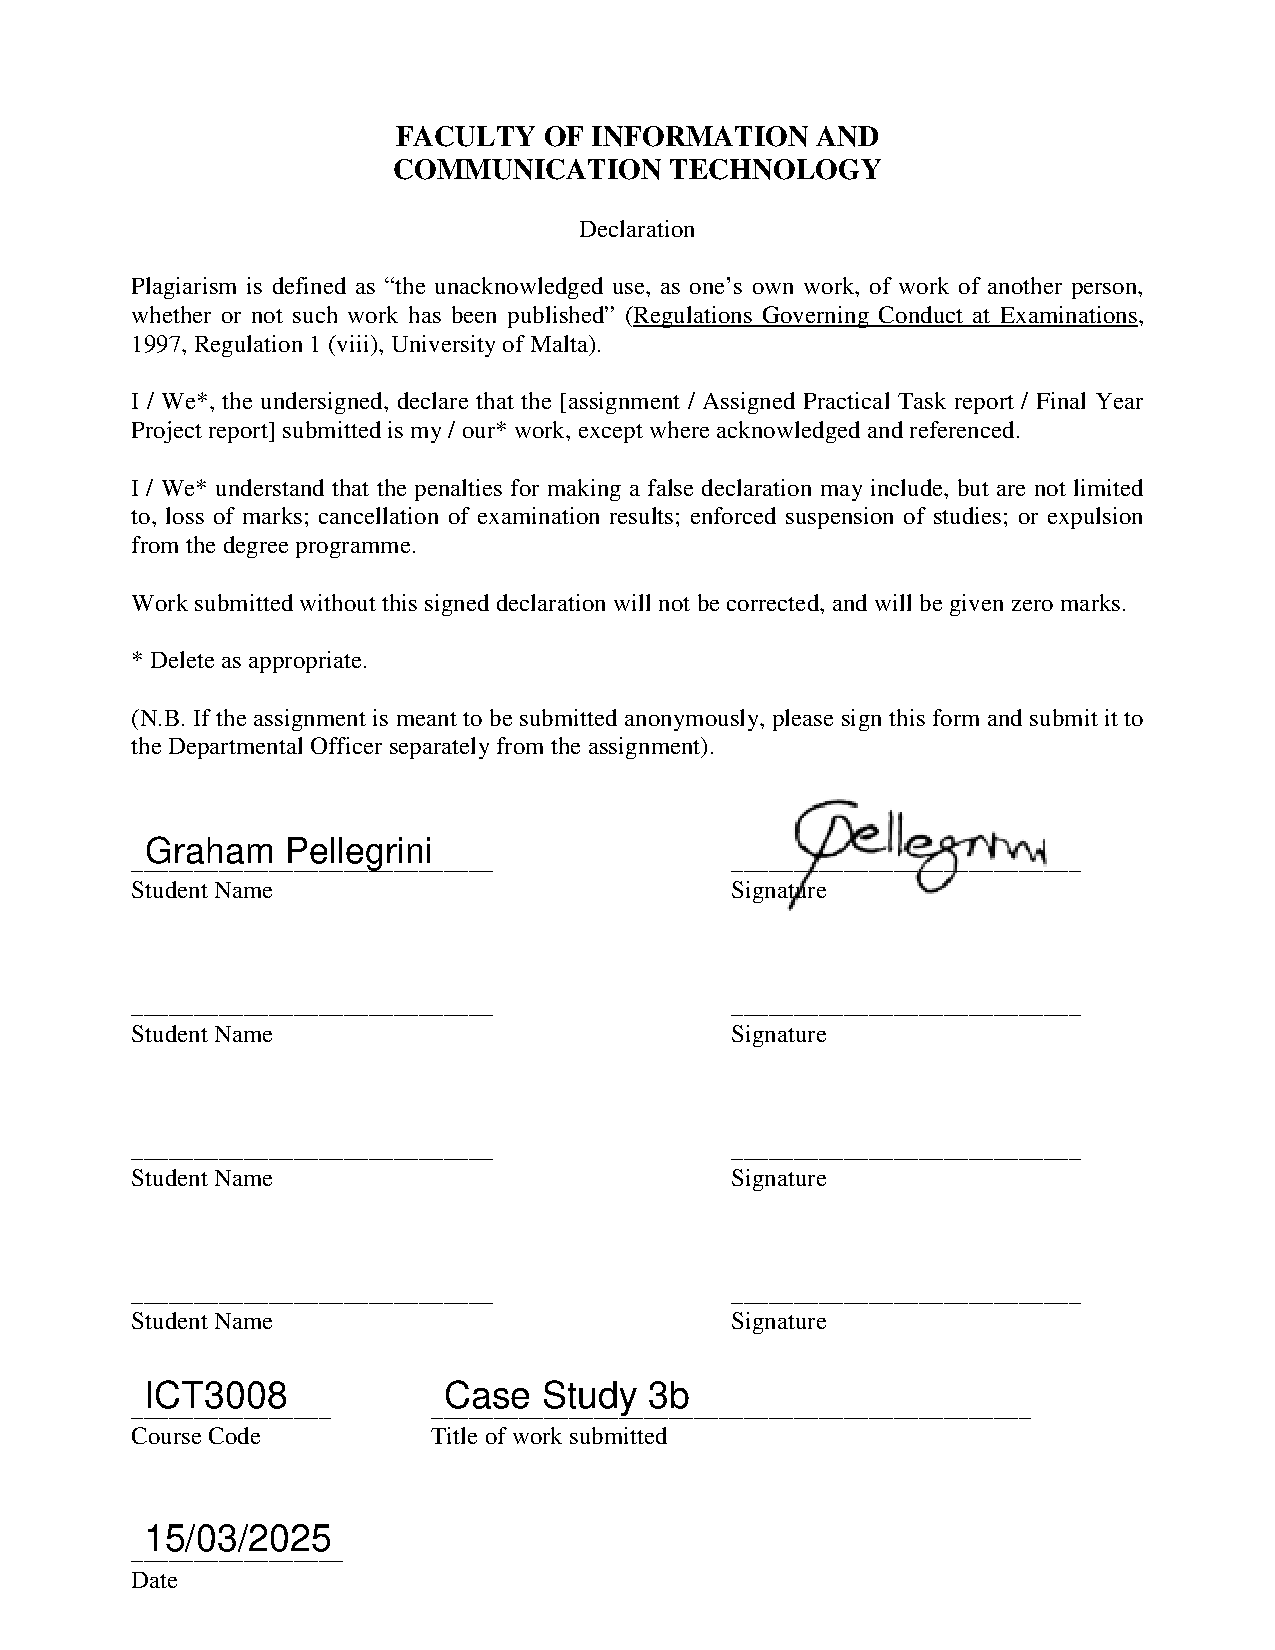
\includepdf[pages=-]{PlagiarismForm.pdf}

\end{document}